\documentclass[10pt,a4paper]{article}
\usepackage[T1]{fontenc}
\usepackage{amsmath}
\usepackage{amsfonts}
\usepackage{amssymb}
\usepackage{graphicx}
\usepackage{enumitem}
\usepackage{titlesec}
\usepackage{geometry}
\geometry{a4paper, margin=1in}
\usepackage{hyperref} 
\usepackage[portuguese]{babel}

% Configurações de títulos para um visual mais limpo e profissional
\titleformat{\section}[block]{\bfseries\Large\raggedright}{}{0em}{}
\titlespacing{\section}{0pt}{1.5em}{1em}

\title{Plano de Formação: Linux - Serviços de Redes}
\author{Formador: [Seu Nome]}
\date{Data de Elaboração: [Data]}


\begin{document}
	
	\section*{Conteúdos}
	
	\subsection*{0. Introdução ao Linux (5 horas)}
	\vspace{-1.2em}
	\paragraph{}
	Antes de explorarmos os serviços de rede, é fundamental entender a filosofia e as ferramentas básicas do Linux.
	
	\begin{itemize}
		\item \textbf{O que é o Linux?} (1 hora) \\
		Explicação simples do sistema operativo, suas principais características (código aberto, seguro, personalizável) e a diferença entre o kernel e uma distribuição (Debian, Ubuntu, Fedora).
		
		\item \textbf{A Magia da Linha de Comando} (2 horas) \\
		Apresentar o terminal como a principal ferramenta de trabalho.
		\begin{verbatim}
			# Navegação básica
			ls -l          # Lista ficheiros e pastas (o -l mostra mais detalhes)
			cd /home       # Navega para a pasta "home"
			pwd            # Mostra o seu diretório atual
			
			# Criar e apagar ficheiros
			touch ficheiro.txt
			rm ficheiro.txt
		\end{verbatim}
		
		\item \textbf{O Conceito de Ficheiros e Diretórios} (2 horas) \\
		Explicação da estrutura hierárquica do Linux (`/`, `/home`, `/etc`, `/var/log`).
		
		\item \textbf{Exercício de Consolidação} \\
		1. Crie uma nova pasta chamada \texttt{treino} na sua pasta pessoal.
		2. Dentro da pasta \texttt{treino}, crie um ficheiro de texto chamado \texttt{notas.txt}.
		3. Use o comando \texttt{ls -l} para confirmar que o ficheiro foi criado.
		4. Apague o ficheiro e, em seguida, a pasta que criou.
	\end{itemize}
	
	---
	
	\subsection*{1. Serviços de rede (10 horas)}
	\vspace{-1.2em}
	\paragraph{}
	Nesta secção, vamos explorar como os serviços de rede são geridos no Linux, desde o seu início até ao encerramento, e os principais ficheiros e diretórios envolvidos neste processo.
	
	\begin{itemize}
		\item \textbf{O Gestor de Tarefas: O Papel do \texttt{systemd}} (3 horas) \\
		Pense no \texttt{systemd} como o "gerente de todas as tarefas" do seu computador. Ele garante que tudo (serviços de rede, servidores web, etc.) comece a funcionar na ordem certa quando o sistema é ligado.
		
		\item \textbf{Controlar Serviços com \texttt{systemctl}} (5 horas) \\
		O comando \texttt{systemctl} é como a "lista de comandos" para o gestor de tarefas.
		\begin{verbatim}
			# Ver o estado de um serviço (Exemplo: SSH)
			systemctl status sshd
			
			# Ligar, desligar e reiniciar um serviço
			systemctl start sshd
			systemctl stop sshd
			systemctl restart sshd
			
			# "Ativar" e "desativar" um serviço para iniciar no arranque
			systemctl enable sshd
			systemctl disable sshd
		\end{verbatim}
		
		\begin{figure}[h]
			\centering
			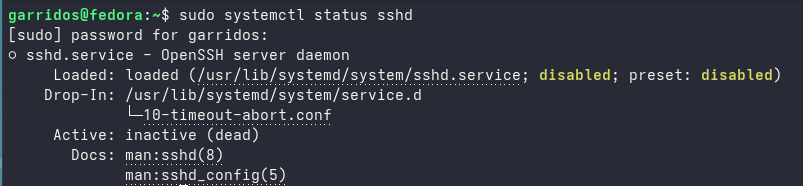
\includegraphics[width=0.8\textwidth]{img/systemctl_status.png}
			\caption{Exemplo da saída do comando \texttt{systemctl status sshd}. \textit{Fonte: Imagem encontrada via Google Images.}}
			\label{fig:systemctl_status}
		\end{figure}
		
		\item \textbf{Exercício de Consolidação} (2 horas)
		1. Instale um servidor web simples (como o Nginx) no seu sistema.
		2. Use \texttt{systemctl status nginx} para verificar se ele está a funcionar.
		3. Desligue-o com \texttt{systemctl stop nginx} e verifique o estado novamente.
		4. Crie um ficheiro de unidade `.service` básico para uma aplicação simples, como um script de "Olá, mundo!" e ative-o para que inicie no próximo arranque.
	\end{itemize}
	
	---
	
	\subsection*{2. XINET.d (4 horas)}
	\vspace{-1.2em}
	\paragraph{}
	O \texttt{xinetd} é como um "rececionista" que só acorda um funcionário (serviço) quando alguém aparece para o ver. Isso economiza energia! É usado para serviços que não precisam estar sempre a funcionar.
	
	\begin{itemize}
		\item \textbf{Configuração e Gestão} (2 horas) \\
		As configurações do \texttt{xinetd} estão nos ficheiros do diretório \texttt{/etc/xinet.d/}. Cada serviço tem o seu próprio "cartão de identificação".
		\begin{verbatim}
			service telnet
			{
				disable         = yes # Para ativar, mude para "no"
				...
			}
		\end{verbatim}
		
		\item \textbf{Exercício de Consolidação} (2 horas) \\
		1. Encontre o ficheiro de configuração do serviço \texttt{ftp} no diretório \texttt{/etc/xinet.d/}.
		2. Altere o valor da opção \texttt{disable} para habilitá-lo.
		3. Reinicie o serviço \texttt{xinetd} para que as alterações entrem em vigor: `systemctl restart xinetd`.
		4. Use um cliente FTP para tentar ligar-se à sua máquina e confirme que o serviço foi ativado.
	\end{itemize}
	
	---
	
	\subsection*{3. TCPWrappers (4 horas)}
	\vspace{-1.2em}
	\paragraph{}
	Pense nos \texttt{TCPWrappers} como um porteiro. Ele decide quem pode entrar (permitir) e quem não pode (negar) num serviço, com base no endereço IP.
	
	\begin{itemize}
		\item \textbf{As Duas Listas: `hosts.allow` e `hosts.deny`} (2 horas) \\
		- \texttt{hosts.allow}: A "lista de convidados". Se alguém estiver aqui, entra.
		- \texttt{hosts.deny}: A "lista negra". Se alguém não estiver na lista de convidados e estiver aqui, é barrado.
		
		\item \textbf{Sintaxe e Exemplos Avançados} (1 hora) \\
		Pode usar `ALL` para todos e `EXCEPT` para criar exceções.
		\begin{verbatim}
			# No ficheiro /etc/hosts.allow
			sshd: 192.168.1.100 EXCEPT 192.168.1.101
			
			# No ficheiro /etc/hosts.deny
			sshd: ALL
		\end{verbatim}
		Neste exemplo, todos podem aceder ao SSH, exceto o IP `192.168.1.101`.
		
		\item \textbf{Exercício de Consolidação} (1 hora) \\
		1. Configure o seu ficheiro \texttt{hosts.deny} para negar o acesso SSH a todos.
		2. No ficheiro \texttt{hosts.allow}, adicione o IP do seu computador para poder aceder.
		3. Tente ligar-se a partir de outro computador para confirmar que o acesso é negado.
	\end{itemize}
	
	---
	
	\subsection*{4. NIS (6 horas)}
	\vspace{-1.2em}
	\paragraph{}
	O NIS é como ter uma única "identidade" para toda uma rede de computadores. Em vez de ter uma conta de utilizador em cada máquina, você tem uma conta num servidor central que funciona em todas as máquinas NIS.
	
	\begin{itemize}
		\item \textbf{Arquitetura NIS (Servidor Mestre e Cliente)} (3 horas) \\
		- \textbf{Servidor Mestre}: Tem a lista principal de utilizadores e grupos.
		- \textbf{Cliente NIS}: Pede ao servidor as informações de utilizadores. O `ypbind` é o serviço que o cliente usa para encontrar o servidor.
		
		\item \textbf{Configuração do Cliente} (2 horas) \\
		Os clientes precisam de saber a que servidor NIS ligar. Isso é definido no ficheiro `/etc/nsswitch.conf`, onde se indica ao sistema para procurar utilizadores e grupos no NIS, além dos ficheiros locais.
		
		\item \textbf{Exercício de Consolidação} (1 hora) \\
		1. Numa máquina cliente, use o comando \texttt{ypwhich} para ver qual é o servidor NIS.
		2. Use \texttt{ypcat passwd} para listar as contas de utilizador.
		3. Crie uma nova conta de utilizador no servidor NIS (o instrutor deve mostrar como) e verifique se consegue iniciar sessão com essa conta a partir do computador cliente.
	\end{itemize}
	
	---
	
	\subsection*{5. DHCP (9 horas)}
	\vspace{-1.2em}
	\paragraph{}
	O DHCP é um protocolo que automaticamente dá um "endereço de rua" (o endereço IP) a cada dispositivo que se liga à sua rede.
	
	\begin{itemize}
		\item \textbf{O Processo DORA: Como funciona?} (4 horas) \\
		Pense no processo DORA como uma conversa entre um novo dispositivo e o servidor DHCP:
		\begin{enumerate}
			\item **D**iscover: "Olá, estou aqui! Há algum servidor DHCP disponível?"
			\item **O**ffer: "Sim, eu sou um servidor! Aqui está um endereço IP que pode usar."
			\item **R**equest: "OK, obrigado! Quero usar este endereço."
			\item **A**cknowledge: "Certo, é todo seu! Divirta-se na rede!"
		\end{enumerate}
		
		\begin{figure}[h]
			\centering
			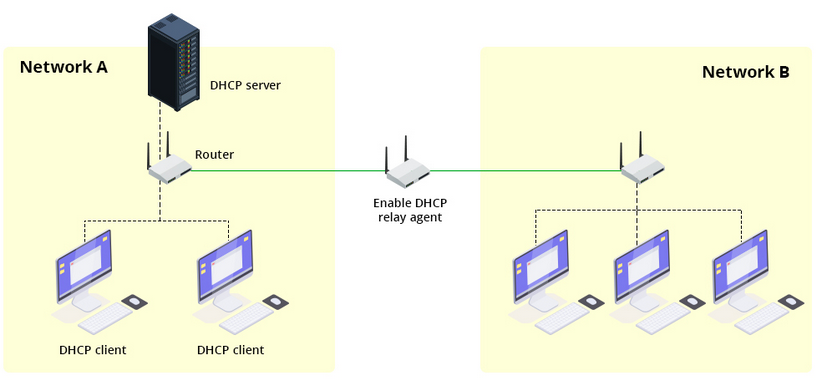
\includegraphics[width=0.8\textwidth]{img/dhcp_dora.png}
			\caption{Diagrama do processo DORA. \textit{Fonte: Imagem encontrada via Google Images.}}
			\label{fig:dhcp_dora}
		\end{figure}
		
		\item \textbf{Configuração e Atribuição de Endereços} (3 horas) \\
		O ficheiro de configuração principal é o \texttt{/etc/dhcp/dhcpd.conf}.
		- \texttt{subnet}: Define a rede que o servidor vai gerir.
		- \texttt{range}: A lista de IPs que serão atribuídos dinamicamente.
		- \texttt{option routers}: Define o endereço do router/gateway.
		- \texttt{host}: Para dar um IP fixo a um computador específico (com base no endereço MAC).
		
		\item \textbf{Exercício de Consolidação} (2 horas) \\
		1. Configure um servidor DHCP para a sua rede de treino com um `range` de IPs para os alunos.
		2. Adicione uma entrada estática para o computador do instrutor, garantindo que ele tenha sempre o mesmo IP.
		3. Reinicie o serviço DHCP e peça aos alunos para testarem se estão a receber os IPs da forma correta.
	\end{itemize}
	
	---
	
	\subsection*{6. DNS (10 horas)}
	\vspace{-1.2em}
	\paragraph{}
	O DNS é como a "lista telefónica" da internet. Ele traduz nomes fáceis de lembrar (como `google.com`) em endereços IP que os computadores entendem (como `142.250.187.110`).
	
	\begin{itemize}
		\item \textbf{Como a Lista Telefónica Funciona: A Hierarquia} (5 horas) \\
		A consulta de DNS é um processo de "perguntas e respostas":
		1.  O seu computador pergunta ao servidor DNS local: "Qual o IP de `google.com`?"
		2.  Se o servidor não souber, ele pergunta ao "servidor de raiz": "Onde encontro o `.com`?"
		3.  O servidor de raiz responde: "Vá ao servidor `.com`."
		4.  O servidor DNS local pergunta ao servidor `.com`: "Onde encontro o `google`?"
		5.  O servidor `.com` responde: "Vá ao servidor autoritativo de `google.com`."
		6.  O servidor DNS local pergunta ao servidor de `google.com`: "Qual o IP de `google.com`?"
		7.  O servidor responde com o endereço IP.
		
		\begin{figure}[h]
			\centering
			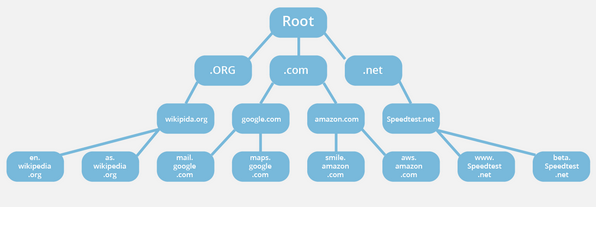
\includegraphics[width=0.8\textwidth]{img/dns_lookup.png}
			\caption{Fluxo de uma consulta DNS típica, mostrando a hierarquia de servidores. \textit{Fonte: Imagem encontrada via Google Images.}}
			\label{fig:dns_lookup}
		\end{figure}
		
		\item \textbf{Tipos de Registos DNS (A, CNAME, MX)} (3 horas) \\
		- \texttt{A}: É a entrada principal, que diz `google.com` -> `142.250.187.110`.
		- \texttt{CNAME}: Cria um "apelido". Exemplo: `www` é um apelido para o servidor principal.
		- \texttt{MX}: Diz qual servidor de email é responsável por um domínio.
		
		\item \textbf{Exercício de Consolidação} (2 horas) \\
		1. Use o comando `dig google.com` para ver a resposta DNS.
		2. Use `dig www.google.com` para ver como o `CNAME` funciona.
		3. Use `dig google.com MX` para encontrar o servidor de e-mail.
		4. Crie um ficheiro de zona simples para um domínio `minhaescola.com` e adicione os registos A, CNAME e MX.
	\end{itemize}
	
	---
	
	\subsection*{7. LOGS (2 horas)}
	\vspace{-1.2em}
	\paragraph{}
	Os logs são como um "diário de bordo" do seu computador. Eles registam tudo o que acontece e são essenciais para encontrar erros e problemas.
	
	\begin{itemize}
		\item \textbf{Onde Encontrar o Diário} (1 hora) \\
		A maioria dos logs está em \texttt{/var/log}. Os ficheiros mais importantes são:
		- \texttt{syslog} ou \texttt{messages}: Mensagens gerais do sistema.
		- \texttt{auth.log}: Registos de login e autenticação.
		
		\item \textbf{Como Ler o Diário: Comandos Úteis} (1 hora) \\
		- \texttt{tail -f /var/log/syslog}: Mostra as últimas linhas do ficheiro e acompanha as novas linhas em tempo real.
		- \texttt{grep "erro" /var/log/syslog}: Procura por uma palavra-chave como "erro".
		
		\item \textbf{Exercício de Consolidação} \\
		1. Tente iniciar um serviço com a sintaxe errada (o instrutor deve mostrar).
		2. Use o comando \texttt{tail} ou \texttt{grep} para encontrar a mensagem de erro no ficheiro de log e identifique o motivo do erro.
		3. Filtre os logs de autenticação para encontrar todas as tentativas de login falhadas na sua máquina.
	\end{itemize}
	
\end{document}